\documentclass{article} % for elife comment
 \usepackage[document]{ragged2e}
\setlength{\RaggedRightParindent}{\parindent}
\setlength{\parskip}{1em}

% \documentclass[9pt
% \item neno]{elife}

\usepackage{geometry} % for elife comment
  \geometry{a4paper, left=32mm, right=32mm, top=30mm, bottom=30mm} % for elife comment

\usepackage[utf8]{inputenc}

\usepackage{lineno} % used along with \linenumbers after begin document. 
\usepackage{setspace} % line spacing
  \setstretch{1.4}
\usepackage{enumitem}
\usepackage{microtype} % Creates better spaced text
\usepackage{siunitx} % SI units 

\usepackage{xcolor} % Setting colours and their usage
  \definecolor{natureblue}{RGB}{5,110,210}

\usepackage[colorlinks]{hyperref} % Colour for hyperlinks, (URLs, citations, cross reference)
  \AtBeginDocument{%this allows colours to change from the defined article template.
  \hypersetup{
  linkcolor={natureblue},
  citecolor={natureblue},
  filecolor=blue!50!black,
  urlcolor=natureblue,
  }}

\usepackage{natbib}
  \setcitestyle{square,numbers,sort&compress}
  \setcitestyle{sort&compress}
\usepackage{hypernat} % hypernat also required to allow citations to compress. 
\usepackage{graphicx}
\graphicspath{ {images/} } % sets the path to image files (Figures)

\usepackage{booktabs} % required for tables
\usepackage{rotating,tabularx} % tabularx is the table style used, rotating can also be used
\newcolumntype{Z}{ >{\centering\arraybackslash}X } % defining table content layout per box
\usepackage{ltablex} % allow page break between lines in tabularx
\usepackage{caption} \captionsetup{font=normalsize} % to set the caption size as normal even when table is tiny.

\usepackage{pdflscape} % for rotated table
\usepackage{multirow} % for table
\usepackage{authblk} % authors
%Define command to start a supplemental section
\newcommand{\beginsupplement}{%
        \setcounter{table}{0}
        \renewcommand{\thetable}{S\arabic{table}}%
        \setcounter{figure}{0}
        \renewcommand{\thefigure}{S\arabic{figure}}%
     }

\usepackage{authblk} % authors
\makeatletter % list affiliations on a single line
\renewcommand\AB@affilsepx{, \protect\Affilfont}

 % left align the title/affiliation section
\renewcommand{\maketitle}{\bgroup\setlength{\parindent}{0pt}
\begin{flushleft}
  \textbf{\@title}

  \@author
\end{flushleft}\egroup
}
\makeatother

\begin{document}
\date{} %don't want date printed
%make title bold and 14 pt font (Latex default is non-bold, 16 pt)
\title{\Large \bf Viral genetic determinants of prolonged respiratory syncytial virus infection among infants in a healthy term birth cohort.
% \footnote{This document's source code is available to co-authors from the  \href{https://github.com/DylanLawless/inspire2022lawless.github.io}{GitHub repository} and from the \href{https://www.overleaf.com/project/61718a4e077acc3d20ee68f1}{overleaf online editor document}.  All code and supplemental live data results at \href{https://github.com/DylanLawless/inspire2022lawless.github.io}{https://github.com/DylanLawless/inspire2022lawless.github.io}. The PDF will be published on  \href{https://www.medrxiv.org}{medrxiv}  before submission. Please note the URL is on my personal domain temporarily; this will be switched for release. For eLife, authors are asked to agree to publish their work under the terms of the Creative Commons Attribution license \href{https://creativecommons.org/licenses/by/4.0/}{CC-BY-4.0}. }
}

% 1 epfl
% 2 penn
% 3 sib
% 4 DIDVan
% 5 emoryPed
% 6 bioVan
% 7 medVan
% 8 DoAVan
% 9 pedVan

\author[1]{\rm Dylan Lawless, PhD}
\author[2]{\rm Christopher G. McKennan, PhD}
\author[3]{\rm Thomas Junier, PhD}
\author[1]{\rm Zhi Ming Xu, MSc}
\author[4]{\rm Suman Das, PhD}
\author[5]{\rm Larry J Anderson}
\author[6]{\rm  Tebeb Gebretsadik}
\author[7]{\rm Meghan Shilts}
\author[8]{\rm Christian Rosas-Salazar}
\author[9]{\rm James D. Chappell, MD}
\author[1]{\rm Jacques Fellay, MD, PhD }
\author[7,9]{\rm Tina V. Hartert, MD, MPH}

\affil[1]{Global Health Institute, School of Life Sciences, École Polytechnique Fédérale de Lausanne, Lausanne, Switzerland}
\affil[2]{Department of Statistics, University of Pittsburgh, Pittsburgh, Pennsylvania, United States of America}
\affil[3]{Swiss Institute of Bioinformatics, Vital-IT Group, Switzerland}
\affil[4]{Division of Infectious Diseases, Department of Medicine, Vanderbilt University Medical Center, Nashville, Tennessee, United States of America}
\affil[5]{Department of Pediatrics, Emory University School of Medicine, Atlanta, Georgia, United States of America}
\affil[6]{Department of Biostatistics, Vanderbilt University Medical Center, Nashville, Tennessee, United States of America}
\affil[7]{Department of Medicine, Vanderbilt University Medical Center, Nashville, Tennessee, United States of America}
\affil[8]{Division of Allergy, Immunology, and Pulmonary Medicine, Department of Pediatrics, Vanderbilt University Medical Center, Nashville, Tennessee, United States of America}
\affil[9]{Department of Pediatrics, Vanderbilt University Medical Center, Nashville, Tennessee, United States of America}

%\affil[ ]{\textit {\{email1,email2,email3,email4\}@xyz.edu}}
\maketitle

% Journal: eLife
% alternates: CID, JID, PLOS pathogens, Journal of virology.

% \linenumbers
\subsection*{Abbreviations}
ALT (alternative);
CI (confidence interval);
GWAS (genome-wide association study);
G (glycoprotein);
H (hemagglutinin);
HN (hemagglutinin-neuraminidase);
IFN (interferon);
IQR (interquartile range);
INSPIRE (The INfant Susceptibility to Pulmonary Infections and Asthma Following RSV Exposure);
LD (linkage disequilibrium);
MAF (minor allele frequency);
MSA (multiple sequence alignment);
OR (odds ratio);
PCR (polymerase chain reaction);
PCA (Principal component analysis);
REF (reference);
RT (reverse transcription);
SVD (singular value decomposition);
SNP (single nucleotide polymorphism);
VE (variance explained);
MSA (multiple sequence alignment);
RSV (respiratory syncytial virus).

\subsection*{Notice of Prior Presentation}
The results of the genome wide association study analyses included in this manuscript were presented during the European Society of Human Genetics Conference in June 2020 in Berlin, Germany, which was held remotely 
\citep{lawless2020genome}.

\section*{*Competing interests}
All authors have completed a conflict of interest form (COI). COI listed:

\section*{*Ethics Statement for Human Subjects Research}
The protocol and informed consent documents were approved by the Institutional Review Board at Vanderbilt University Medical Center (\#111299).  
One parent of each participant in the cohort study provided written informed consent for participation in this study. 
The informed consent document explained study procedures and use of data and biospecimens for future studies, including genetic studies.

\section*{*Reviewer suggestion}
Authors are required to provide suggestions for at least four potential reviewers of the work during the Full Submission. eLife reviewer search:
\url{https://datastudio.google.com/embed/u/0/reporting/7ee3012b-8543-4141-9f8e-03355dbfff55/page/OPij}.

%
%Name
%Institution
%Country
%Keywords
%Webpage

%Meike Dittmann
%New York University Grossman School of Medicine
%United States of America
%virology, interferons, innate immunity, viral-host interactions, antiviral defenses, human airway epithelium
%dittmannlab.com
%
%Charlotte Houldcroft
%University of Cambridge
%United Kingdom
%virus genomics, herpesviruses, molecular epidemiology, adna
%https://www.infectiousdisease.cam.ac.uk/directory/ch504@cam.ac.uk
%
%Emily Davenport
%Penn State University
%United States of America
%microbiome, gwas, genomics, gene expression
%https://davenport-lab.github.io/
%
%Philip Ashton
%Malawi Liverpool Wellcome
%Malawi
%microbiology, genomics, bioinformatics, global health, diarrhoea, salmonella, tb
%https://scholar.google.co.uk/citations?user=JPi-2JAAAAAJ&hl=en
%
%Danna Gifford
%The University of Manchester
%United Kingdom
%experimental evolution, genomics, antibiotic resistance, theoretical evolution
%https://dannagifford.com
%
%R Blake Billmyre
%Stowers Institute for Medical Research
%United States of America
%genome evolution, fungal pathogenesis, genomics, quorum sensing, hypermutation
%https://research.stowers.org/zanderslab/lab-members/blake-billmyre.html
%
%Lin Wang
%University of Cambridge
%United Kingdom
%infectious disease modeling, computational biology, data science, bayesian statistics, machine learning, immunology, pathogen evolution
%https://www.gen.cam.ac.uk/directory/lin-wang
%
%Julia Steinberg
%The Daffodil Centre, The University of Sydney
%Australia
%genetics, genomics, epidemiology, risk prediction, disease susceptibility, precision public health, large data analysis
%https://orcid.org/0000-0002-0585-2312
%
%Cesar Fortes-Lima
%Uppsala University
%Sweden
%human population genetics, biological anthropology, genomics, natural selection
%http://katalog.uu.se/profile/?id=N18-1379
%
%Daniel Blanco-Melo
%Fred Hutchinson Cancer Research Center
%United States of America
%paleovirology, innate immunity, interferons, host-virus interactions, molecular arms race
%https://research.fredhutch.org/blanco-melo/en.html

\clearpage
\section{Abstract}
\textbf{Background}: Respiratory syncytial virus (RSV) is primarily associated with acute respiratory infection, however, many RNA viruses can establish prolonged or persistent infection in some infected individuals.

\textbf{Objectives}: To identify viral genetic variants associated with prolonged infection and determine if there are host genetic risk alleles for first RSV infection risk.

\textbf{Methods}: In a population-based cohort study of healthy term infants, RSV infection was determined by biweekly surveillance for RSV and 1-year RSV serology. Using RSV whole-genome sequencing, viral amino acids (genotype) were tested for association with 
% \textit{a priori} defined 
prolonged infant RSV infection adjusting for host features associated with increased infection risk. We tested the association of infant RSV infection risk with severe RSV and childhood asthma-associated SNPs.

\textbf{Results}: A significant viral genetic association in the RSV G protein, p.E123K/D and p.P218T/S/L, identified as candidate causal variants associated with prolonged infection after Bonferroni correction for multiple testing. These variants were associated exclusively with upper respiratory tract infection, and on average, milder clinical infection compared with other circulating variants. We found no evidence of host genetic risk for RSV infection.

\textbf{Conclusions}: We identified a novel RSV viral variant associated with prolonged infection in healthy infants and no evidence supporting host genetic susceptibility to first RSV infection during infancy. As the capacity of RSV for chronicity and its viral reservoir are not understood, these results are of fundamental interest in understanding viral and host genetic contributions that may underlie the development of chronic respiratory morbidity.

\section{Introduction}
Respiratory syncytial virus (RSV), a \textit{Human orthopneumovirus}, is the single most important respiratory virus to infant global health, resulting in significant morbidity and mortality in infants 
\citep{hall_burden_2009}.
By the age of two to three years, nearly all children are infected with RSV at least once 
\citep{glezen_risk_1986}.
RSV is a seasonal mucosal pathogen that infects primarily the upper and lower respiratory tract epithelium, although it has been recovered from non-airway sources 
\citep{bokun_respiratory_2019,
cubie_detection_1997,
nadal_isolation_1990,
odonnell_respiratory_1998,
rezaee_respiratory_2011,
rohwedder_detection_1998}.
RSV is primarily associated with acute respiratory infection, however, many RNA viruses can establish prolonged or persistent infection in some infected individuals. [refs] 
Prolonged shedding of RSV, especially in young infants and following first infection, has been demonstrated, with longer average duration of viral shedding using polymerase chain reaction (PCR) to detect RSV 
\citep{munywoki_influence_2015}.
While younger age and first infection are associated with protracted infection [ref], 
what is not understood is whether there are viral factors contributing to prolonged RSV shedding or infection in infants. 
This is important, as prolonged infection or shedding may contribute to enhanced transmission and developmental changes to the early life airway epithelium. 
Further, the reservoir of RSV infection is not understood, 
and it is possible that some RSV strains could populate a dormant reservoir for infection that is activated by seasonal or other influences 
\citep{hobson_persistent_2008}.

The objectives of this study were to identify viral genetic variants associated with ``prolonged infection'' and determine if there are host genetic risk alleles for first RSV infection risk. 
These questions are of fundamental interest in understanding viral and host genetic contributions that may underlie the development of chronic respiratory morbidity.

To determine if there is evidence of host genetic factors for risk of infant RSV infection we tested the association of $\approx 60$ severe RSV and childhood asthma-associated single nucleotide polymorphisms (SNPs) in a population-based cohort of term healthy infants.
We also conducted a host GWAS to identify common variants associated with infant RSV infection, and narrow sense heritability to test for small cumulative effects. 
We \textit{a priori} defined the clinical entity of ``prolonged'' infection during infancy as those with repeat positive PCR separated by 15 or more days and who repeatedly met pre-specified criteria for an acute respiratory infection
\citep{okiro2010duration}.
RSV genome sequencing was done on all isolates meeting illness criteria with positive RSV PCR. 
Viral amino acids (genotype) of the F and G glycoprotein were tested for association with ``prolonged'' infection adjusting for host features associated with increased infection risk. 
We focused our analyses on the surface F (fusion) and G (attachment) proteins of RSV as they have been implicated in pathogenesis \citep{boyoglu2015anti,bukreyev2012secreted}, 
and both are targets for neutralizing antibodies during infection
\citep{anderson1988neutralization, ngwuta2015prefusion}.
Lastly, to determine if the variants of interest were enriched by selective pressure over time, we used public data from the past three decades to assess variant frequency over time.

\section{Methods}
\subsection{Study population}
The protocol and informed consent documents were approved by the Institutional Review Board at Vanderbilt University Medical Center (\#111299).  
One parent of each participant in the cohort study provided written informed consent for participation in this study. 
The informed consent document explained study procedures and use of data and biospecimens for future studies, including genetic studies.

The study population is a longitudinal birth cohort - The INfant Susceptibility to Pulmonary Infections and Asthma Following RSV Exposure (INSPIRE) - specifically designed to capture the first RSV infection for term healthy infants. 
Additional details of this birth cohort have been previously published 
\citep{larkin_objectives_2015}.
Briefly, the cohort includes 1952 term ($\ge$ 37 weeks gestation), non-low birth weight ($\ge$ 2250 g, 5 lbs), otherwise healthy infants from a population-representative sample of pediatric practices located in a rural, suburban, and urban regions of the southeastern US during 2012-2014. 
Infants were born June through December so that they would, by design, be 6 months of age or less entering their first RSV season. 

\subsection{Biweekly surveillance of RSV infection}
Infant (i.e., the first year of life) RSV infection was ascertained through passive and active biweekly surveillance during each infant's first RSV season and RSV serology
(Table \ref{tab:1}).
If an infant met pre-specified criteria for an acute respiratory infection, we then conducted an in-person respiratory illness visit at which time we administered a parental questionnaire, performed a physical exam, collected a nasal wash, and completed a structured medical chart review for infants seen during an unscheduled visit. 
Viral identification in nasal samples was done by reverse transcription-quantitative PCR for RSV
\citep{larkin2015objectives}. 
% [Plots with CT-value from Tina, either as supplemental or first mention later so not to pollute the order]. 
We defined ``prolonged'' infections as those among infants with positive PCR separated by 15 or more days and repeatedly met pre-specified criteria for an acute respiratory infection 
(Figure \ref{fig:1}).
Viral genetic analyses were then conducted on this set of infants.

\subsection{Descriptive analyses}
Descriptive analyses of the cohort were conducted using R 4.0.5 (available at: 
\url{http://www.r-project.org}). 
Pearson or Wilcoxon tests were used for comparing infants with and without prolonged RSV infection.
The main descriptive features are provided in 
Table \ref{tab:1}.
% [Consider plotting these also in the Hmisc Harrell style as seen in his book, RegerssionModellingStrategies2015].

\subsection{Host DNA Collection and Genotyping}
One-year blood samples were selected based on availability of DNA among a random group of children and genotyped with the Multi-Ethnic Global Array microarray (Illumina, CA, United States) at the University of Washington DNA Sequencing and Gene Analysis Center.

\subsection{Genetic Analyses of RSV Infection in Infancy}
A GWAS was performed on 621 children with available DNA for the association between host genotype and RSV infection during infancy.
Due to sample size constraints we also restricted our sub-analysis to the $\approx 60$ RSV LRTI- and childhood asthma-associated host SNPs identified in 
\citet{pividori2019shared, janssen2007genetic, pasanen2017genome}, 
respectively, to test the association of infant RSV infection risk (as defined by RSV infection detected through biweekly surveillance or RSV serology) with known childhood asthma- or RSV bronchiolitis-associated single nucleotide polymorphisms.
%[refs]
We additionally evaluated the accumulation of small genetic effects that would go undetected in a GWAS by estimating the heritability of RSV infection. 

For GWAS analyses, the initial round of data quality control was performed on individual populations (self-reported as White, Black, and  Hispanic) using PLINK version 1.9 
\citep{purcell2007plink}.
Subjects with a missing genotype call rate of 5\% were removed. 
The single nucleotide polymorphism (SNP) minor allele frequency (MAF) threshold was set for cohorts as MAF $> $ 0.01, 0.03, 0.08 for White, Black, and Hispanic, respectively
\citep{liu2016dbnsfp}.
The groups were merged for a total of 1,086,830 variants and a genotyping rate of 0.78. 
Subject independence was assessed using KING (\url{https://people.virginia.edu/~wc9c/KING/}) to prevent spurious associations. 
However, no probable relatives or duplicates were detected based on pairwise identify-by-state. 
We compared the genetic ancestry in cases to self-reported ethnicity to check for mislabeling.
Reported and estimated sex was also examined for discrepancy.
Next, a second round of quality control on the combined dataset was conducted, which removed 74 samples due to genotype missingness and 399,991 variants with a genotyping rate $< 0.1$. 
Samples were checked for departure from Hardy-Weinberg equilibrium (HWE) (P $< 1e^{-6}$) to uncover features of selection, population admixture, cryptic relatedness, or genotyping error. 
This was only performed on controls to prevent removal of genuine genetic associations that can be associated with this measurement, removing 6,024 variants. 
No variants had a MAF $< 0.01$ after merging.
% Note: We did not use the imputed dataset for the final analysis, to simplify the data especially for subset analysis of known GWAS SNPs.
% Genotyping data was phased [SHAPEIT2] \url{https://mathgen.stats.ox.ac.uk/genetics_software/shapeit/shapeit.html} and imputed [IMPUTE2] \url{https://mathgen.stats.ox.ac.uk/impute/impute_v2.html} using the 1000 Genomes Project phase 3 reference panel. The reference genome build and LD population used was hg19/1000G Nov2014 EUR. Imputation quality was assessed and SNPs with an information score of $<0.8$ or minor allele frequency $<0.05$ were removed.
SNP positions and identifiers were compared and updated according to dbNSFP4.0a (hg19) with 289 variants removed due to a missing coordinate and SNPs identifier
\citep{liu2016dbnsfp}.
This resulted in an analysis-ready dataset of 680,526 variants from 621 children (509 and 112 with and without RSV infection in infancy, respectively) with a total genotyping rate of 0.98. 
No genomic inflation was evident with an estimated lambda (based on median chi-squared test) equal to 1. 
We then used genome-wide complex trait analysis (GCTA) software (\url{https://cnsgenomics.com/software/gcta/}) to calculate the genetic relationship matrix and performed principal component analysis to account for population structure
\citep{yang2011gcta}.
Genome-wide association analysis was performed using PLINK version 1.9 for logistic regression with multiple covariates that included the child's birth month, enrollment year (as a marker of RSV season), daycare attendance, the presence of another child $\le 6$ years of age at home, sex, and 6 ancestry principal components as covariates
\citep{purcell2007plink}.
Due to the multiple testing burden likely precluding our ability to identify small genetic effects in our GWAS, we conducted additional heritability analyses.

For the heritability analyses, we used the method described by Golan et al to estimate the narrow-sense heritability of RSV infection infancy on the latent liability scale ($h_l^2$), which, if  $> 0$, would indicate an accumulation of small genetic effects
\citep{golan2014measuring}.
We estimated $h_l^2$ to be exactly 0, suggesting that, if present, infant RSV infection-related genetic signals are both small and sparse. 

\subsection{RSV whole-genome sequencing}
RSV whole-genome sequencing of this study population has been previously described 
\citep{schobel_respiratory_2016}.
Briefly, RNA was extracted at J. Craig Venter Institute (JCVI) (\url{https://www.jcvi.org}) in Rockville, MD from nasal wash samples which were RSV PCR positive and collected during a respiratory illness visit triggered through biweekly surveillance of symptoms. 
Four forward reverse-transcription (RT) primers were designed and four sets of PCR primers were manually picked from primers designed across a consensus of complete RSV genome sequences using JCVI’s automated primer design tool
\citep{li_automated_2012}.
cDNA was generated from \SI{4}{\micro\liter}  undiluted RNA, using the pooled forward primers and SuperScript III Reverse Transcriptase (Thermo Fisher Scientific, Waltham, MA, USA). 
100 ng of pooled DNA amplicons were sheared to create 400-bp libraries, which were pooled in equal volumes and cleaned. 
For samples requiring extra coverage, in addition to Ion Torrent sequencing, Illumina libraries were prepared using the Nextera DNA Sample Preparation Kit (Illumina, Inc., San Diego, CA, USA). 
Sequence reads were sorted by barcode, trimmed, and de novo assembled using CLC Bio's \textit{clc\_novo\_assemble} program, and the resulting contigs were searched against custom, full-length RSV nucleotide databases to find the closest reference sequence. 
All sequence reads were then mapped to the selected reference RSV sequence using CLC Bio's \textit{clc\_ref\_assemble\_long} program 
\citep{bioWhite2016}.
% <!-- \citep{bioWhite2010} redundant v3.0 removed to reduce citations -->
Curated assemblies were validated and annotated with the viral annotation software called Viral Genome ORF Reader, VIGOR 3.0 (\url{https://sourceforge.net/projects/jcvi-vigor/files/}), before submission to GenBank as part of the Bioproject accession PRJNA225816 (\url{https://www.ncbi.nlm.nih.gov/bioproject/225816})
% <!--(30-Oct-2013 73 samples)-->
\citep{wang_vigor_2012} 
and PRJNA267583 (\url{https://www.ncbi.nlm.nih.gov/bioproject/267583}).
% <!--(17-Nov-2014 264 samples)-->

\subsection{Viral Sequence alignment}
% <!---_Sequence data format:_--->
% <!---sqn--->
The NCBI-tools Tbl2asn (\url{https://www.ncbi.nlm.nih.gov/genbank/tbl2asn2/})
was used in the creation of sequence records for submission to GenBank (\url{https://www.ncbi.nlm.nih.gov/genbank/}).
A total of 350 viral sequences in \textit{.sqn} file format were used for downstream analysis.

% <!---_Fasta format:_--->
% <!---fa--->
We computed a phylogenetic tree for each gene, as follows.
NCBI-tools asn2fsa (\url{https://www.huge-man-linux.net/man1/asn2fsa.html}) was used to to convert to fasta format.
% <!--- /work/gr-fe/lawless/inspire/rsv_viral_seq/ 1.export_nucleotide.sh --->
% <!--- 2.simplify_header.sh --->
% <!---_Data curation:_--->
% <!---seg_master/ Mar 3rd--->
Each sample consisted of 11 sequence segments
(NS1, NS2, N, P, M, M2-1, M2-2, SH, G, F, and L) as shown in 
Figure \ref{fig:1}.
These were separated and repooled to create 11 single fasta files for each gene containing all 350 samples. 
% <!---split_seg.sh --->
% <!---With awk, I split each fasta to a new file and labeled with the real name. i.e. segment 1 for all samples is in the file seg\_1, etc. dir: ./seg--->
Sequences were checked so that they would be at least 90\% as long as the maximum length 
for the corresponding gene in order to minimize the loss of aligned positions when computing the phylogenetic tree. 
% <!---_Multiple seuqnce alignment:_--->
% <!---aln/ Feb 18th--->
Each of the eleven resulting sets was aligned with MAFFT v7 (\url{https://mafft.cbrc.jp/alignment/software/})
\citep{katoh2013mafft},
using default  parameters.
The sequence of the orthologous gene from  \textit{Bovine orthopneumovirus} 
(\href{https://www.ncbi.nlm.nih.gov/nuccore/NC_001989}{GenBank:NC\_001989}) 
was added to each set as an outgroup. 
% <!---
%pep (outgroup seq)
%msa (all aligned per gene)
%pep (fixed version of msa)
%--->
% <!---  clw/ Jan 28th (Muscle alignment) Not used by Thomas --->
% <!--- nex/ Jan 30thI don't think this was used.  One nexus file per gene. It stores information about taxa, morphological and molecular characters, distances, genetic codes, assumptions, sets, trees, etc. --->

% <!---_Phylogenetic tree:_--->
% <!---nw/ Mar 10th--->
IQ-Tree 
(\url{https://www.iqtree.org})
\citep{nguyen2015iq}
was used with per-gene multiple sequence alignment (MSA) files for estimating maximum-likelihood phylogenies.
% <!---Analysis results written to:
%IQ-TREE report:                M2-2_new_wOG.msa.iqtree¬
%Maximum-likelihood tree:       M2-2_new_wOG.msa.treefile¬
%Likelihood distances:          M2-2_new_wOG.msa.mldist¬
%Screen log file:               M2-2_new_wOG.msa.log¬
%msa
%msa.bionj
%msa.ckp.gz
%msa.iqtree
%msa.log
%msa.mldist
%msa.model.gz
%msa.treefile
%msa.uniqueseq.phy 
%--->
% <!---_Alignment Quality:_--->
Examining the sequences with an alignment viewer showed that a small number of sequences had frame-shift variants but these did not affect the regions included in our testing criteria.
% <!--Discuss whether anything extra is needed for these sequences; e.g. alignments recomputed until no frame shifts were observed.-->
% <!---
%\subsection{Analysis order of code}
%1. update_G_phylogeny_nucleic_acid_msa_logist_data_prep_covariates.R
%2. update_G_phylogeny_nucleic_acid_msa_logist_covariates.R source(1)
%3. update_G_pca.R source(1+2)
%4. update_G_LD source(1)
%5. asthma_and_candidate_variant_lm (no sig results, remove)
%6. public_data
%--->

% <!-- ## Data merged and cleaned -->
% <!--Label repeat infections -->
Viral sequence data and clinical information were merged and cleaned with R.
Clinical IDs matching more than one viral sequence ID were used to re-identify samples from the same individual as prolonged infections. 
Genetic variation was quantified in these samples and for subsequent analysis only the first viral sequence was included for association testing. 
Antigenic grouping of strain A and B had been completed previously and labels were included to annotate each sample accordingly.

The cohort-specific variant frequency per position was calculated;
residues were counted and ranked by frequency
with the most frequent residue defined as reference (REF) and alternative (ALT) for variants.
Positions with at least one ALT were checked for potential misalignment or other sources of error. 
Variant positions were selected for association analysis, while non-variant position were ignored.

A number of host features have been previously shown to influence infection susceptibility and were therefore included as covariates in our analysis 
\citep{rosas2022upper}.
Six samples were excluded due to insufficient covariate data, resulting in 344 test samples. 
Of these, 38 were from the same patients (prolonged or repeat infection) of which half (19) were included for association testing; 325 samples total.
% <!--Correlations viewed with: corrplot, ggcorrplot, caret.-->

\subsection{Population structure}
The genetic distances to nearest neighbors were computed based on phylogenetic 
trees generated with MAFFT.
% [Other methods also used but not pertinent; include some info from the code].
Principal component analysis (PCA) and singular value decomposition (SVD) were used in dimensionality reduction for exploratory data analysis of viral phylogeny.
R package \textit{factoextra} was used for PCA, and to visualise eigenvalues and variance. 
R package \textit{caret} was used to analyse genetic correlations.

\subsection{Association testing}
Viral amino acids (genotype collapsed into REF/ALT) were tested for association with infection types \textit{single} and \textit{prolonged}, 
including key covariates that are significantly associated with infection.
Analysis was performed using logistic regression with the
R stats (3.6.2) \textit{glm} function as a generalized linear model.
The model consisted of the binary response (prolonged infection Yes/No), and predictors - viral genotype (REF/ALT amino acid), viral PCs 1-5, host sex, and accounted for host features that have been previously demonstrated as significantly associated with infection: 
self-reported race/ethnicity, child-care attendance, living with siblings 
\citep{rosas2022upper}.

% $ glm(\text{Infection status} \text{\textasciitilde} \text{genotype} + \text{PCs} + \text{birth month} + \text{sex} + \text{race} + \text{child-care} + \text{siblings}, \text{family} = \text{'binomial'}) $

The environmental host covariates did not contribute any significant effect in our model for the candidate-causal association.
Five viral PCs were included in our model to account for population structure.
% [Check the \% VE from PC scree plot stats to 1 decimal place and list it here.]
Bonferroni correction for multiple testing was applied based on the number of independent variants tested.
R package \textit{stats} was used for a range of analyses including glm for logistic regressions. 
R package \textit{MASS} was used to analyse logistic regression model data.
% <!-- 
%\subsection{Strain definition and sub-analysis}
%Put sub-strain analysis into supplemental.
%Do we want to include anything else being done with this cohort?;
%RT-PCR, 
%serology, and genomic. 
%Strain sub-analysis.
%-->
% Second infections occurred mostly in those with strain B. 
To test if the significantly associated variants were due to population structure, 
a subset of only strain B was performed. 
% In result instead; Due to the smaller sample size the result no longer passed the significant threshold. 
% However, the same direct of effect indicated that the association was not a false positive. 
% OR and CI. 
% <!--
%\subsection{Variance over time in public data}
%-->

\subsection{Biological interpretation}
%Some but not all of these methods will be included for our results section. 
% Adjust based on discussion with co-authors.
Infant RSV infection results in decreased barrier function of the airway epithelium
\citep{connelly2021metabolic}.
Association between interferon (INF)-$\gamma$ and RSV amino acid position (W=wild type versus A=alternatives) was adjusted for the same covariates as the main analysis.
% Wilcoxon test comparing IFN-$\gamma$, and IFN-$\alpha$, between RSV amino acid positions (W= wild type vs A=alternatives [3 combined]).
Protein structures were analysed with data sourced from 
RCSB PDB \url{https://www.rcsb.org}.
% (Define the choice of PDB used - refer to R script). 
Protein function and domains were assessed using 
UniProt	(\url{https://www.uniprot.org})
for P03423 (GLYC\_HRSVA) (strain A2) and O36633 (GLYC\_HRSVB) (strain B1) in gff format:
% uniprot_RSV_GLYC_HRSVA_P03423.gff
\url{https://www.uniprot.org/uniprot/P03423} and
% uniprot_RSV_GLYC_HRSVB_O36633.gff
\url{https://www.uniprot.org/uniprot/O36633}, respectively.
Interactions, PTM, motifs, and epitopes were assessed from literature. 
%* Domain blast. 
%* Multiple organism alignment - not complete.
Protein features were assessed using data from NCBI
(\url{https://www.ncbi.nlm.nih.gov/ipg/NP_056862.1}) and
via sequence viewer with O36633.1 human RSV B1, 
(\url{https://www.ncbi.nlm.nih.gov/projects/sviewer/?id=O36633.1})
Potential effects of amino acid variation on protein structure and function were considered according to available information on a broad range of biological and biochemical features, including native conformation (secondary, tertiary, and quaternary), domains and topology, disulfide bonds, glycosylation, interactions with other viral proteins and host-cell factors, proteolytic cleavage sites, normal patterns of intra- and/or extra-cellular distribution, and secretion status.

\paragraph{IFN response section?}

\section{Results}
\subsection{Cohort characteristics}
The INSPIRE cohort consisted of 1,949 enrolled infants 
(Figure \ref{fig:1}).
Of these, 1,220 ($\sim 63\%$) had $\ge$ 1 in-person respiratory illness visit(s). 
In total, there were 2,093 in-person respiratory illness visits completed and the median (interquartile range [IQR]) number of in-person respiratory illness visits per infant was 1 (1-2).
From the cohort, 344 RSV viral samples from 326 individuals were sequenced.
Prolonged infection was \textit{a priori} defined as RSV sequence positive with $\ge$ 15 days between testing and meeting criteria for acute respiratory infection.
There were 19 infants who met the definition of prolonged infection with viral genetic analysis used to confirm clonality of original and subsequent virus detections. 
Table \ref{tab:1} lists the cohort characteristics of infants with prolonged RSV infection compared with other RSV infection and the entire cohort. 

The relatively small sample size of our cohort required analysis that targeted only genes which were \textit{a priori} likely to functionally contribute to the clinical phenotype. 
Therefore, our analysis focused on the F and G glycoprotein. 
% (citations probably not required: PMC8310105, 33115881, 23598484, 31533056).
% <!-- [Include some points for our reasoning; -->
% <!-- Would we have false positives in other genes? -->
% <!-- We can interpret the results in F and G. -->
% <!-- These are the surface proteins that are most studied for vaccine development etc. -->
% <!-- Variation in other genes is lower; quantify this. --> 
% <!-- G and SH are variable more than others. -->
% <!-- M2 also has a fair amount of sequence variation. --> 
% <!-- F is more variable than others but maybe not the most so. --> 
% <!-- * Surface, entry, targets of immune response. --> 
% <!-- * F - Primary candidate for vaccine. --> 
% <!-- * Biological plausability is higher than others. --> 
% <!-- * G surface "glycoprotein", F - careful with terms. -->
% <!-- Larry / Suman can help. -->
% <!-- Their clinical relevance.] -->

\begin{figure}[ht] \hspace*{0cm}  \begin{center}
    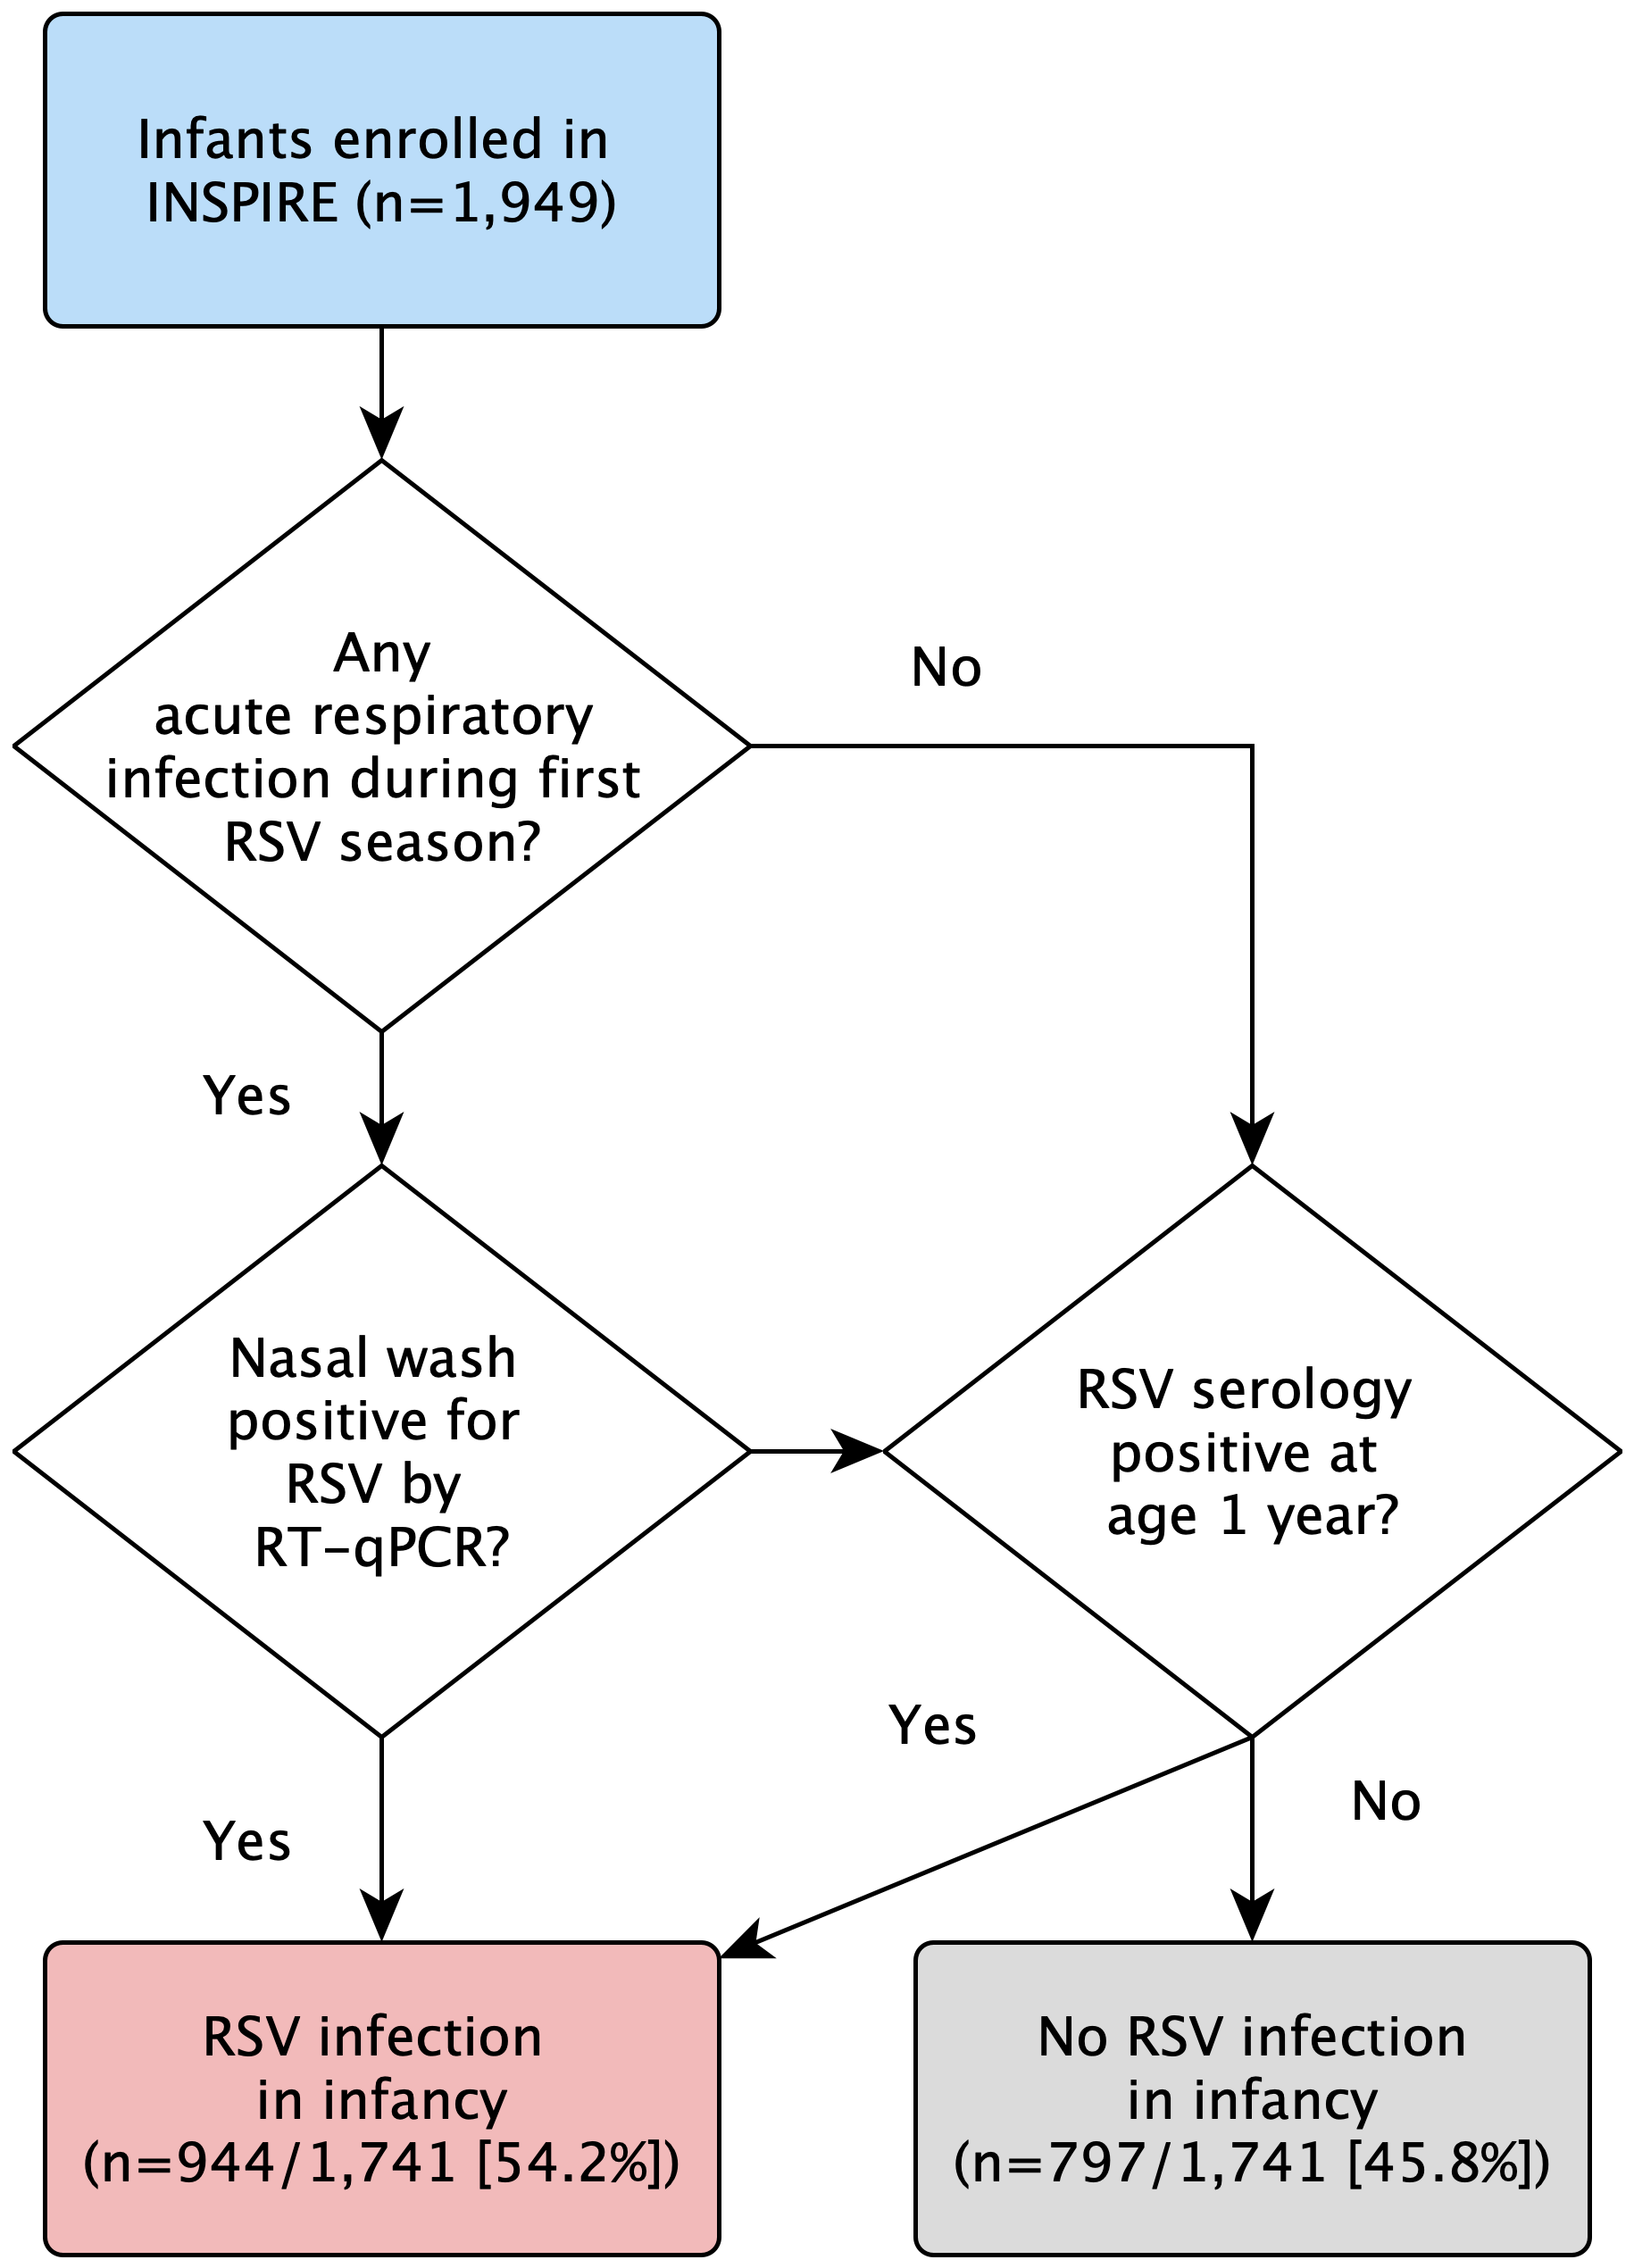
\includegraphics[scale=0.1]{f1_rsv_persist2022}
	\caption{\textbf{Cohort characteristics of infants with prolonged RSV infection compared with other RSV infection and entire cohort}. Prolonged infection is defined as RSV sequence positive, with $\ge 15$ days between testing and meeting criteria for acute respiratory infection. Respiratory severity score (median, IQR). Test statistic $P = 0.27$. Pearson, Wilcoxon.}
	\label{fig:1}
 \end{center} \end{figure}
 
  \begin{landscape}										
\begin{table}[ht]										
\centering										
\begin{tabularx}{\linewidth}{ X l X X X X }										
\toprule										
{		} & {		} & {	Prolonged RSV N=19	} & {	Other RSV N=342	} & {	Total N=1949	} \\
\midrule										
\multirow{2}{*}{	Illness	} &{	Illness age, months (median, IQR)	} & {	6 (4, 6) 	} & {	4 (2, 5)	} & {	NA	} \\
{		} &{	Respiratory severity score (median, IQR)	} & {	2.0 (1.2, 3.0)	} & {	3.0 (2.0, 4.0)	} & {	NA	 } \\
\midrule										
\multirow{2}{*} {	RSV season	} & {	2012-13	} & {	68\%	} & {	54\%	} & {	44\%	} \\
{		} & {	2013-14	} & {	32\%	} & {	46\%	} & {	56\%	} \\
\midrule										
\multirow{4}{*}{	Self reported Race	} & {	Non-Hispanic Black	} & {	37\%	} & {	13\%	} & {	18\%	} \\
{		} & {	 Non-Hispanic White	} & {	63\%	} & {	69\%	} & {	65\%	} \\
{		} & {	 Hispanic	} & {	0\%	} & {	10\%	} & {	9\%	} \\
{		} & {	 Multi-race/ethnicity/other 	} & {	0\%	} & {	8\%	} & {	8\%	} \\
\midrule										
\multirow{2}{*}{	Sex	} & {	Female	} & {	53\%	} & {	44\%	} & {	48\%	} \\
{		} & {	 Male	} & {	47\%	} & {	56\%	} & {	52\%	} \\
 \midrule										
\multirow{2}{*}{	Second-hand smoke exposure	} & {	No	} & {	79\%	} & {	77\%	} & {	53\%	} \\
{		} & {	Yes	} & {	21\%	} & {	23\%	} & {	47\%	} \\
\midrule										
 \multirow{3}{*}{	Insurance	} & {	Medicaid	} & {	68\%	} & {	48\%	} & {	54\%	} \\
{		} & {	Private	} & {	32\%	} & {	51\%	} & {	45\%	} \\
{		} & {	None/unknown	} & {	0\%	} & {	1\%	} & {	1\%	} \\
\midrule										
 \multirow{2}{*}{	Daycare/Sibling*	} & {	No	} & {	16\%	} & {	22\%	} & {	34\%	} \\
{		} & {	Yes	} & {	84\%	} & {	78\%	} & {	66\%	} \\
\bottomrule										
\caption{										
\textbf{Cohort characteristics of infants with prolonged RSV infection compared with other RSV infection and entire cohort}. 										
Prolonged infection is defined as RSV sequence positive, with $\ge$15 days between testing and meeting criteria for acute respiratory infection. *Presence of sibling or another child $\le$ 6 years of age at home.}										
\label{tab:1}										
\end{tabularx}										
\end{table}										
\end{landscape}										

\clearpage										

\subsection{Host Genetic Analyses}
We explored whether RSV infection in infancy (or the lack thereof) is a natural assignment (quasi-random) event and, unlike the severity of early-life RSV infection,
\citep{larkin2015genes}
not determined by host genetics. 
For the candidate-SNP analysis, we considered childhood asthma- and RSV bronchiolitis-associated SNPs identified in 
\citet{pividori2019shared, janssen2007genetic, pasanen2017genome}.
The first is the largest childhood asthma GWAS to date, and, as far as we are aware, the latter 2 represent the most comprehensive studies of RSV bronchiolitis-associated SNPs. 
To further reduce the multiple testing burden, we only analyzed SNPs with MAF$\ge 0.1$ in at least one of the White, Black, or Hispanic ethnicity groups. 
The associations between the genotype at the resulting 54 SNPs (50 childhood asthma- and 4 RSV bronchiolitis-associated SNPs) and RSV infection in infancy in our data are given in 
\textbf{Figure} \ref{fig:host_genetics}
which suggests that the genotype at these SNPs have little to no effect on RSV infection in infancy. 
We further investigated the possibility that we were underpowered to observe associations with these SNPs by pooling information across SNPs to estimate the average genetic effect size. 
In brief, we computed a z-score for each SNP, where the average (across SNPs) squared z-score $\bar{G}$ is proportional to the average squared genetic effect on RSV infection in infancy. 
As $\bar{G}$ is an average of $p=54$ approximately independent statistics, 
it is approximately
$N(n\mu^2 + 1,2/p)$
where $n=621$ is the sample size and $\mu^2$ is a function of the average squared genetic effect on RSV infection in infancy. 
Using the genetic effect estimates from 
\citet{pividori2019shared, janssen2007genetic, pasanen2017genome}
we calculated that we would have 80\% power to reject the global null hypothesis of no genetic effect on RSV infection in infancy at any of these SNPs (i.e. $\mu^2 =0$) if, on average across the 54 SNPs, the genetic effect on RSV infection in infancy was at least 61\% as large as those estimated in the aforementioned 3 studies. 
We found $\bar{G}$=1.00 in our data, which corresponds to a p-value of 0.50. 
This result indicates that the genetic effect on RSV infection in infancy is zero or small at SNPs \textit{a priori} likely to be associated with RSV infection.	

\begin{figure}[ht] \hspace{-0.5cm}
\begin{center}
    \includegraphics[scale=0.07]{host_genetics}
\end{center} 
	\caption{\textbf{Genetic analyses of RSV infection in infancy}.
		(A) The Manhattan plot shows no genome-wide significant associations (p-value threshold of $5e^{-8}$).
		(B) The Q-Q plot demonstrates that the observed p-values are congruent with those expected under the null hypothesis that RSV infection in infancy is independent of genotype. 
		(C) The association between the 54 selected childhood asthma- or RSV bronchiolitis-associated SNPs and RSV infection in infancy in our data. 
		The solid red line is the identity line, and the dashed grey lines are $/pm 1$ standard deviation around the expected -log10(p-value). 
		The results suggest that the genotype at these SNPs have little to no effect on RSV infection in infancy. 
		RSV: respiratory syncytial virus; SNP: single nucleotide polymorphism.
	}
	\label{fig:host_genetics} 
\end{figure}
\clearpage

\subsection{Population structure}
A summary of protein coding genes in RSV is illustrated in
Figure \ref{fig:2} A.
Our analysis focused on G protein, as indicated.
The phylogenetic tree based on multiple sequence alignment (MSA) of G protein amino acid sequences is shown in 
Figure \ref{fig:2} B.
One obvious feature causing a separation in genetic diversity is G protein partial gene duplication, 
which has emerged in recent years within RSV-A strains 
\citep{eshaghi2012genetic}.
RSV-B strains with an analogous duplication have existed for two decades, 
although the selection process leading to emergence and clinical implications have not been entirely defined.

We observed prolonged infections by viruses from different phylogenetic clades, rather than one specific clade 
(Figure \ref{fig:2} C).
A genotype correlation matrix and PCA eignenvalues were used for reducing the dimensionality of sequence data.
Dimension one accounted for 95.19\% cumulative variance explained in our cohort.
All other dimensions account for very little variance, which is evenly distributed; no particular protein coding sequence separated the cohort.
          % <!-- eigenvalue variance.percent cumulative.variance.percent -->
% <!-- Dim.1   1.608637e+02     9.518559e+01                    95.18559 -->
For his reason, in our main analysis, viral population structure was accounted for by the first five principal components (PC). 
Three PCs are shown in Figure \ref{fig:2} C.
To test for type I errors due to the population structure between strain A and B, 
a subset analysis of individual strains was performed to confirm the validity of the combined analysis downstream.
% <!-- The main analysis was also repeated using viral strain labels A and B (separately derived from the clinical laboratory testing) instead of PCs which did not alter the analysis results, indicating no errors in sample handling. --> 

% Note for presentation slides: there is no general theoretical reason that the most informative linear function of the predictor variables should lie among the dominant principal components of the multivariate distribution of the predictor variables. 
% However, if there were then we would like to know since it would produce a false positive in this case. Conversely, for example, in a principal component regression you would hope to find the assoc based on PCs.

\subsection{Genetic invariance of prolonged infection}
The duration of RSV shedding in Kenyan infants has been reported previously
\citep{okiro2010duration}.
 % <!-- \url{https://bmcinfectdis.biomedcentral.com/articles/10.1186/1471-2334-10-15#Sec1} -->
% <!-- This is the follow up. Ask Tina about the first paper too. --> 
Based on these findings, infections separated by at least 15 days were expected to be ``new'' infections. 
% <!-- In addition to our within-cohort genetic analysis showing --> 
Figure \ref{fig:2} D (panel [i]) summarises every pairwise genetic distance between every viral sequence.
Sequence from the same clades have the smallest distance; panel [ii] shows genetic invariance between viral sequences within the same host for infections separated by at least 15 days. 
There was no significant genetic variation in prolonged viral sequence within individuals versus significantly increased genetic diversity between any of the most closely related sequences ($\text{P-value} = 0.008$).
Panel [iii] shows distances between all possible pairs within clades ($\text{P-value} = 1.3e^{-8}$).
We therefore refer to these cases as prolonged infection rather than reinfections.
% <!-- Have a look at update figure but the first version might be fine. --> 

\begin{figure}[ht] \hspace{-0.5cm} 
    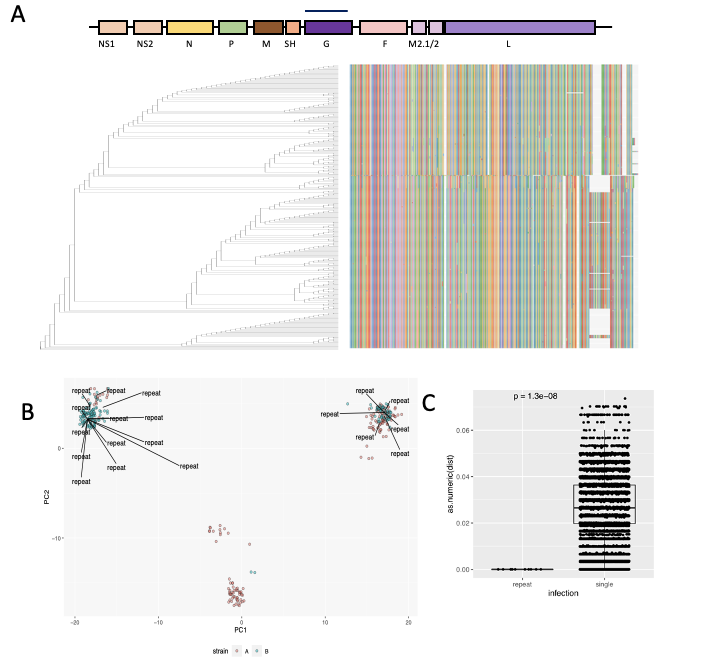
\includegraphics[scale=0.8]{f2}
	\caption{\textbf{Population structure}.
(A) Protein coding genes in RSV.
(B) Phylogenetic tree based based on multiple sequence alignment (MSA) of G protein amino acid sequences.
(C) Principal component analysis (PCA) PCs1-3 with labels indicating prolonged infections from different phylogenetic clades.
(D) Panel [i] summarises every pairwise genetic distance between every viral sequence.
Genetic invariance in prolonged infections separated by at least 15 days compared to other genetic variation within clades  
(panel [ii]) and within all possible pairs (panel [iii]).}
	\label{fig:2} 
\end{figure}
\clearpage

\subsection{Variants in G glycoprotein significantly associated with prolonged infection}
The consensus sequence within the cohort was assigned based on the major allele.
Variants at the amino acid level were defined as either reference (REF) or alternative (ALT) and assessed for their association with persistence.
The model consisted of 
the binary response (prolonged infection Yes/No),
and predictors; viral genotype (REF/ALT amino acid), viral PCs 1-5, host sex, and host features that have been previously demonstrated as significantly associated with infection;
self-reported race/ethnicity, child-care attendance, or living with siblings
\citep{hall1976respiratory}.
% NB don't jettison this citation.
Analysis was performed using R stats (3.6.2) \textit{glm} function. 
% <!-- glm ( infection ~ genotype + PCs + sex + other). -->
A significant genetic association was identified for prolonged infection after Bonferroni correction for multiple testing (threshold for number independent variants $< 0.05/23 = 0.002$), 
as shown in 
Figure \ref{fig:3} A. 
Since many variants within RSV coding genes have non-random association due to selection, like linkage disequilibrium (LD) in human GWAS, 
we reduced the multiple testing burden by retaining proxy variants and removing those with
$r^2 \ge 0.8$.

To determine whether this association was simply due to population stratification between strains A and B, a subset analysis was performed using independently assessed clinical laboratory strain labels for A and B.
% <!-- Show how strains are defined in the genome sequence. --> 
% <!-- ## Shown not just false positive, accounting for population structure and strain, --> 
The same direction of effect indicated that the association was not a false positive, although the smaller sample size means that sub-analysis result no longer passes the significant threshold. 
% State the OR in same direction with overlapping SE.

To assess the possibility of a false positive due to population structure within our cohort,
we assessed the magnitude of variance explained (VE) at every amino acid position.
Figure \ref{fig:3} B (panel [i]) shows the variance explained by each individual variant in PCs1-5.
The values are illustrated according to protein position in panels [ii-iii].
The lead association variant had 
$-0.996\%$ VE for PC1 and $-1.66\%$ VE for PC2,
a negligible effect that precludes spurious association by allele frequency between populations.

After identifying a significant association with prolonged infection,
we quantified the correlation of variants with the lead proxy.
% <!-- Conditional analysis was used to identify any independant signal. --> 
% <!-- Pruning, go through methods with Chris multiple test correction with threshold set at number of proxy SNVs rather than gene-wide SNV number. -->
Clumping was performed with ranking based on MAF and with a cut-off threshold of $r^2 \ge 0.8$ (Supplemental Figure \ref{fig:S1}).
The association model was repeated for all variants to produce a LocusZoom-style Manhattan plot with $r^2$ by color and P-value statistics as shown in 
Figure \ref{fig:3} C.
This shows G protein 
% <!-- "V126" --> 
p.E123K/D and 
% <!-- "V221" --> 
p.P218T/S/L as candidate causal variants associated with prolonged infection. 
No other variants were correlated with this outcome. 

To determine whether p.E123K/D and p.P218T/S/L variant genotypes are novel and potentially influence viral fitness, we searched  the public viral data repository of NCBI \textit{Human orthopneumovirus}, taxid:11250, which contained data from 
27 unique countries worldwide, sample collection dates from 1956 onward, and 1084 glycoprotein protein sequences after curation.
The variants were present at a low and stable frequency, without obvious temporal enrichment. 
Thus, while historical data reveal no positive selective advantage attached to p.E123K/D and p.P218T/S/L, longstanding circulation and linkage in prolonged RSV infection suggest that these polymorphisms are present in the viral inoculum and do not arise through recurrent mutational events.

\subsection{Functional interpretation}
Cell-attachment proteins of paramyxoviruses (G protein in RSV) span the viral envelope and form spike-like projections from the virion surface. 
RSV G protein is a type II integral membrane protein consisting of 298 amino acid residues comprising N-terminal cytoplasmic (p.1-43), transmembrane helical (p.43-63), and extracellular (p.64-298) domains 
(Figure \ref{fig:3} D). 
RSV G protein ectodomain also exists in a soluble secreted form, p.66 – 298, which functions in immune evasion 
\citep{levine1987demonstration, feldman1999identification, feldman2000fusion}.
G protein interacts with the small hydrophobic (SH) protein 
\citep{rixon2005respiratory}
and, via the N-terminus, with matrix (M) 
\citep{ghildyal2005interaction} 
protein.
It has also been reported to form homo-oligomers 
\citep{collins1992oligomerization}.
The variant amino acid positions associated with prolonged infection reside in a portion of the ectodomain of unassigned specific function and linearly non-contiguous with sequences that bind cell-surface heparan sulfate, which likely promotes RSV cell-attachment (p.187-198)
\citep{levine1987demonstration, feldman1999identification, feldman2000fusion}.
In addition, these positions do not contribute to known neutralization epitopes on G protein. Information available in PDB was insufficient to infer effects of p.E123K/D and p.P218T/S/L on local or regional protein structure. 

\begin{figure}[ht] \hspace{-0.5cm} 
    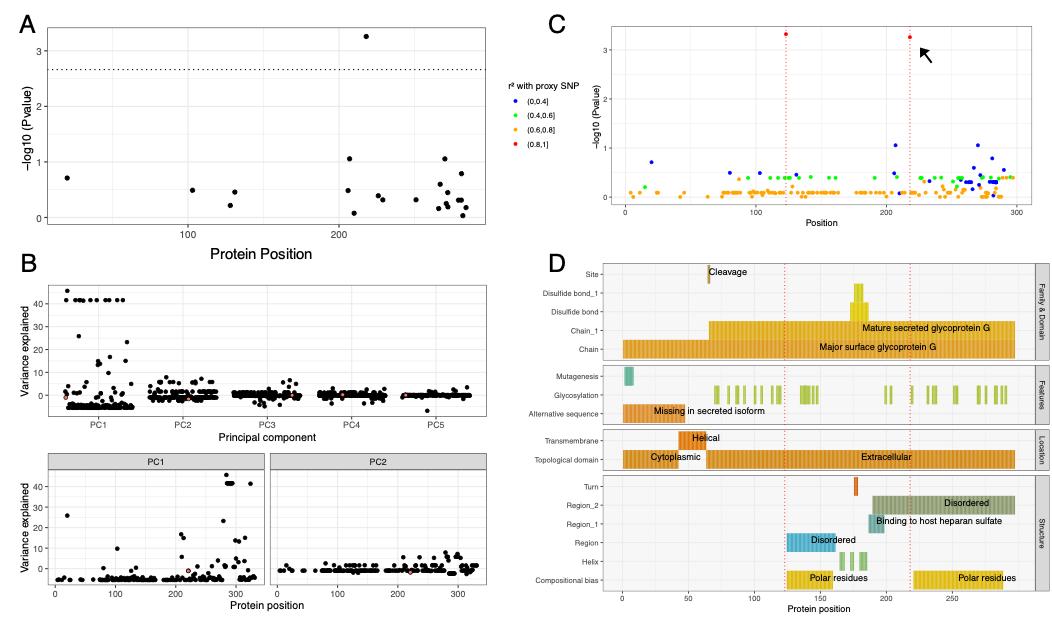
\includegraphics[scale=0.85]{f3}
	\caption{\textbf{Viral genetic association with prolonged infection}. (A) Amino acid association with prolonged infection after multiple testing correction (significant threshold shown by dotted line). (B) Variance explained (VE) within cohort. The effect of each variant on cohort structure is shown for PCs1-2. A large \% VE for a significantly associated variant would indicate a false positive. (C) Variants in strong correlation were clumped for association testing using proxies for $r^2 \ge 0.8$. One significant association was identified (shown in A); the $r^2$ values for all other variants show a single highly correlated variant with the lead proxy (red). 
	(D) Evidence for biological interpretation for every amino acid position is summarised}
	\label{fig:3}
\end{figure}
\clearpage

\subsection{Host response}
Prolonged infections associated with G protein variants p.E123K/D and p.P218T/S/L were on average less severe compared with other circulating variants, and all were limited to the upper respiratory tract(Table \ref{tab:1}). 
Therefore, we analyzed nasal wash samples collected during acute RSV infection for a panel of cytokines involved in antiviral immune responses and observed differential IFN$\alpha$ and IFN$\gamma$ levels segregating according to viral antigenic group—A or B.
Both cytokines were elevated in group [x] infections compared to group [y].
As prolonged infections with p.E123K/D and p.P218T/S/L genotypes were exclusively group [?], 
the dichotomous relationship of IFN$\alpha$ and IFN$\gamma$ levels to antigenic group precluded evaluation of G protein variants as independent predictors of IFN$\alpha$ and IFN$\gamma$ production. 
We reviewed records of p.E123K/D and p.P218T/S/L genotypes in public databases and found that these variants [do/do not] occur preferentially in group A or B strains, which suggests that [insert conservative statement about possible contribution of variant sequences to prolonged infection depending on whether published sequences display group bias].  
% I am unsure how much effort would be required to extract this information, assuming it exists in published records. I included provisional text for consideration as a section fortifier if potential impact justifies the data mining.

% Since the viral strains correlated with the presence of the variants of interest, co-linearity meant that it was not possible to attribute these variants as the cause of a differential interferon response.
% The more pronounced antiviral response is unlikely to be due to the variants associated with prolonged infection and more likely due to other features that separate strain A and B

\section{Discussion}
In this study of term healthy infants, we identified a significant viral genetic association in the RSV G protein of candidate causal variants associated with prolonged infant RSV infection. These variants were not associated with severe disease, had not arisen as a recent mutation, and have been present in public sequence data at a low prevalence for decades. Demonstrating that there is no evidence of host genetic susceptibility for risk of infection with RSV during infancy allowed our analysis to focus on the viral genetic features which may drive prolonged infection without requiring adjustment for host factors. The variant associated with prolonged infection in our cohort is in the extracellular region, and there are no known mechanistic features that directly overlap, although it is possible that variant positions approximate sequences that bind a putative viral receptor, heparan sulfate \citep{feldman1999identification}, in the G protein three-dimensional structure.  As neither the capacity of RSV for prolonged infection in immunocompetent hosts nor the viral reservoir has been delineated,  these results are of fundamental interest in understanding viral and host genetic contributions that may underlie the development of chronic respiratory morbidity.
Although this study was not designed to define mechanisms underlying the association of G protein variants with prolonged infection, we hypothesize that these sequence changes dampen antiviral immune responses and thereby delay viral clearance. We do not expect a role for immune memory in these first-in-life RSV infections; however, we cannot exclude modulatory effects of maternal antibody. 

%\subsection{Cytokines}
We observed differences in the acute antiviral response between subjects with resolved and prolonged infection, specifically, [state difference with respect to IFN in nasal secretions] — but causal inference about variant sequences is co-founded by co-linearity of these polymorphisms with RSV antigenic group. Results of nasal cytokine analysis are nevertheless consistent with a contemplated role for altered immune responses in extended infections by G protein variant strains. 
The possibility of viral mutational immune escape has been reported for 
infants who struggle to control primary RSV infections, allowing for prolonged viral replication and not previously described viral rebound
\citep{brint2017prolonged}.

Strains harboring G protein p.E123K/D and p.P218T/S/L variants might be cleared more slowly and foster an immune environment of low-level chronic stimulation or exhaustion. 
We previously demonstrated that infants infected with RSV in their first year of life have dampened subsequent antiviral immune responses in early childhood \citep{chirkova2022effect} as well as changes in airway epithelial cell metabolism \citep{connelly2021metabolic}.

% Within-host variation with \textit{de novo} mutation may allow variants to present within some individuals but failing to persist within the population, however, we have not been able to conclusively assess this possibility.
Public data show the consistent presence of G protein p.E123K/D and p.P218T/S/L variants at low frequencies [insert frequency range here?] over the past 30 years, without evidence of enrichment by positive selective pressure over time. Yet, why such variants have maintained a stable but low frequency in the human population for decades is unclear. These strains are a potential reservoir, emerging seasonally in response to immune, environmental, or other forces. Alternatively, the polymorphisms might recurrently emerge \textit{de novo} during infection of some individuals but are poorly transmissible because of suboptimal fitness. 

%\subsection{functional interpret}
G protein p.E123K/D and p.P218T/S/L variants are not part of known antibody neutralization epitopes or CD8+ cytotoxic T-cell epitopes (Figure \ref{fig:3}). In addition to heparan sulfate, interactions between viral G protein and CX3CR1, the receptor for the CX3C chemokine fractalkine, have been reported to modulate the immune response and facilitate infection
\citep{levine1987demonstration, feldman1999identification, feldman2000fusion, johnson2015respiratory, tripp2001cx3c, jeong2015cx3cr1}.
Furthermore, the mature secreted isoform of G protein (p.66-298) is thought to facilitate viral antibody evasion by acting as an antigen decoy and modifying the activity of leukocytes bearing Fc-gamma receptors \citep{bukreyev2008secreted}. Our findings raise the interesting prospect that G protein variants associated with prolonged infection alter a key interaction at the immune interface between pathogen and host.

%\subsection{limitations}
While this study has a number of significant strengths, including one of few population-based surveillance studies of first RSV infections during infancy among term healthy infants, our findings are also subject to some limitations. First, this study was not designed with primary intention to examine infection duration, and repeat sampling following initial RSV infection was performed based on criteria for an acute respiratory infection. Asymptomatic prolonged infections would not have been captured. Second, our study cohort was small, necessitating focus on viral surface glycoproteins, F and G, due to their variability and presumed likelihood of a positive association. A larger cohort with serial sampling would be required to diminish the impact of co-linearity of viral genotypes with antigenic groups and to perform informative viral whole genome analysis. Genome-wide information might elucidate other determinants of prolonged infection or pathogen fitness that mediate and/or modulate effects of phenotype-driving variations. Third, again due to small sample size, we could not investigate host genetic risk for prolonged infection. While we have not specifically assessed subjects for rare monogenic variants that may cause an underlying immunodeficiency, our enrollment criteria included only infants who were term and otherwise healthy. 

%\subsection{asthma}
A host genetic interaction for asthma has been demonstrated previously 
\citep{moffatt2010large}.
We performed an interaction analysis for the outcome of host asthma, host genetics, and pathogen genetics 
but no significant interaction was found. 
However, our sample size is unlikely to be sufficient to answer this question, 
which may be addressed with future studies. 

In summary, we identified a novel RSV viral variant associated with prolonged infection in healthy infants, but no evidence of host genetic susceptibility to infant RSV infection. Understanding host and viral mechanisms that contribute to prolonged infection will be important in crafting strategies to control the short- and long-term impact of RSV infection. The identification of RSV variants associated with prolonged infection might also improve vaccine design, particularly if these variants stimulate robust immunity or, in contrast, escape the immune response or induce immunopathologic conditions. The growing availability of large genomic and functional data sources provides opportunities for understanding pathogenesis of infant RSV infection, contribution of viral genetic variants to acute and chronic illness, and pathways to effective vaccines.



\section{Links}
\subsection{Software}
\begin{description}[noitemsep]

\item R v4.1.0 was used for data preparation and analysis \url{http://www.r-project.org}.
\item R package \textit{caret} was used for analysis: genetic correlations.
\item R package \textit{dplyr} was used for data curation.
\item R package \textit{factoextra} was used for analysis: PCA, and to visualise eigenvalues and variance.
\item R package \textit{ggplot2} was used for data visualisation.
\item R package \textit{MASS} was used to analysis: logistic regression model data.
\item R package \textit{stats} was used for analysis: including glm for logistic regressions. 
\item R package \textit{stringr} was used for data curation.
\item R package \textit{tidyr} was used for data curation.
\item asn2fsa \url{https://www.huge-man-linux.net/man1/asn2fsa.html}
\item clc\_novo\_assemble \href{https://resources.qiagenbioinformatics.com/manuals
/clcgenomicsworkbench/852/index.php?manual=De_novo_assembly.html}{qiagenbioinformatics.com} \
\item Clustal Omega \url{https://www.ebi.ac.uk/Tools/msa/clustalo/}
\item dbNSFP (database) \url{http://database.liulab.science/dbNSFP} \citep{liu2016dbnsfp}
\item GCTA \url{https://cnsgenomics.com/software/gcta/} \citep{yang2011gcta}
\item GenBank \url{https://www.ncbi.nlm.nih.gov/genbank/}
\item IQ-Tree \url{https://www.iqtree.org/} \citep{nguyen2015iq}
\item KING \url{https://people.virginia.edu/~wc9c/KING/} \citep{manichaikul_robust_2010}
\item MAFFT \url{https://mafft.cbrc.jp/alignment/software/} \citep{katoh2013mafft}
\item NextAlign \url{https://github.com/nextstrain/nextclade}
\item PLINK \url{http://zzz.bwh.harvard.edu/plink/} \citep{purcell2007plink}
\item Tbl2asn \url{https://www.ncbi.nlm.nih.gov/genbank/tbl2asn2/}
\item Viral Genome ORF Reader, VIGOR 3.0 \url{https://sourceforge.net/projects/jcvi-vigor/files/}
\item RCSB PDB \url{https://www.rcsb.org}
\item UniProt \url{https://www.uniprot.org}

\end{description}

\subsection{Data sources}
\begin{description}[noitemsep]
\item Dataset \url{https://www.ncbi.nlm.nih.gov/bioproject/267583}.
\item Dataset \url{https://www.ncbi.nlm.nih.gov/bioproject/225816}.
\item J. Craig Venter Institute \url{https://www.jcvi.org}.
\item GenBank:NC\_001989 \textit{Bovine orthopneumovirus}, complete genome \url{https://www.ncbi.nlm.nih.gov/nuccore/NC_001989}.
\item Reference data \url{https://www.ncbi.nlm.nih.gov/gene/?term=1489824}.
G attachment glycoprotein [\textit{Human orthopneumovirus}]; ID: 1489824; Location: NC\_001781.1 (4675..5600); Aliases: HRSVgp07.
\item Reference data \url{https://www.ncbi.nlm.nih.gov/gene/?term=37607642}. 
G attachment glycoprotein [\textit{Human orthopneumovirus}]; ID: 37607642; Location: NC\_038235.1 (4673..5595); Aliases: DZD21\_gp07.
\item Reference data for all public NCBI Virus 
\url{https://www.ncbi.nlm.nih.gov/labs/virus/vssi/} for species: \textit{Human orthopneumovirus}; genus: \textit{Orthopneumovirus}; family: \textit{Pneumoviridae}.
\item Reference data \url{https://www.ncbi.nlm.nih.gov/labs/virus/vssi/#/virus?SeqType_s=Nucleotide&VirusLineage_ss=Human\%20orthopneumovirus,\%20taxid:11250}
- contains sequence data for 
Virus Lineage ss=\textit{Human orthopneumovirus}, taxid:11250
nucleotide: 26’965, 
protein: 53’804, 
RefSeq Genomes: 2.
\item Reference \url{https://www.ncbi.nlm.nih.gov/protein/NP_056862.1}
\item GCF\_002815475.1	(release 2018-08-19) Nucleotide Accessions: NC\_038235.1, protein: Y\_009518856.1
\item Reference \url{https://www.ncbi.nlm.nih.gov/protein/YP_009518856.1}
\item GCF\_000855545.1	(release 2015-02-12) Nucleotide Accessions: NC\_001781.1, protein: NP\_056862.1 (strain B1).
\end{description}
% <!-- 73 samples, we would like the accessions for the other samples if possible. -->
% <!-- https://www.ncbi.nlm.nih.gov/nuccore?term=PRJNA225816&cmd=DetailsSearch -->

\section{Code availability}
Public upload of analysis code to GitHub \url{https://github.com/DylanLawless/}.
Do you want a stand-alone repository that we will abandon, or is it OK in my personal page?

\bibliographystyle{unsrtnat}
\bibliography{references}

%%%%%%%%%%%%%%%%%%%%%%%%%%%%
%%%% Supplemental       %%%%
%%%%%%%%%%%%%%%%%%%%%%%%%%%%

\beginsupplement
\section{Supplemental}
 \label{sec:Supplemental_text}
									
\begin{figure}[ht] \hspace{-0.5cm} 
    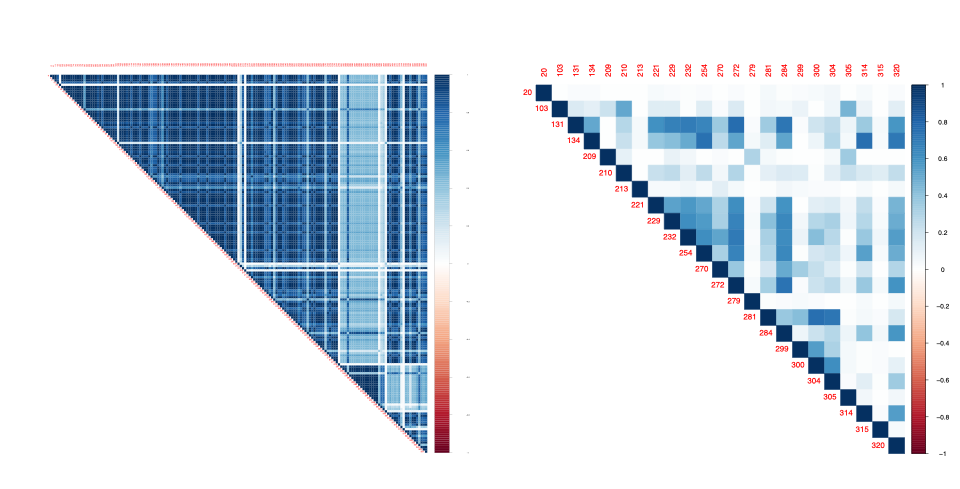
\includegraphics[scale=0.85]{S1}
	\caption{\textbf{Supplemental: Variant clumping for reduction in association testing}. [Left] Correlation between all positions. [Right] Correlation between proxy variants are clumping to remove $r^2 \ge 0.8$.}
	\label{fig:S1}
\end{figure}


\begin{figure}[ht] \hspace{-0.5cm} \begin{center}
    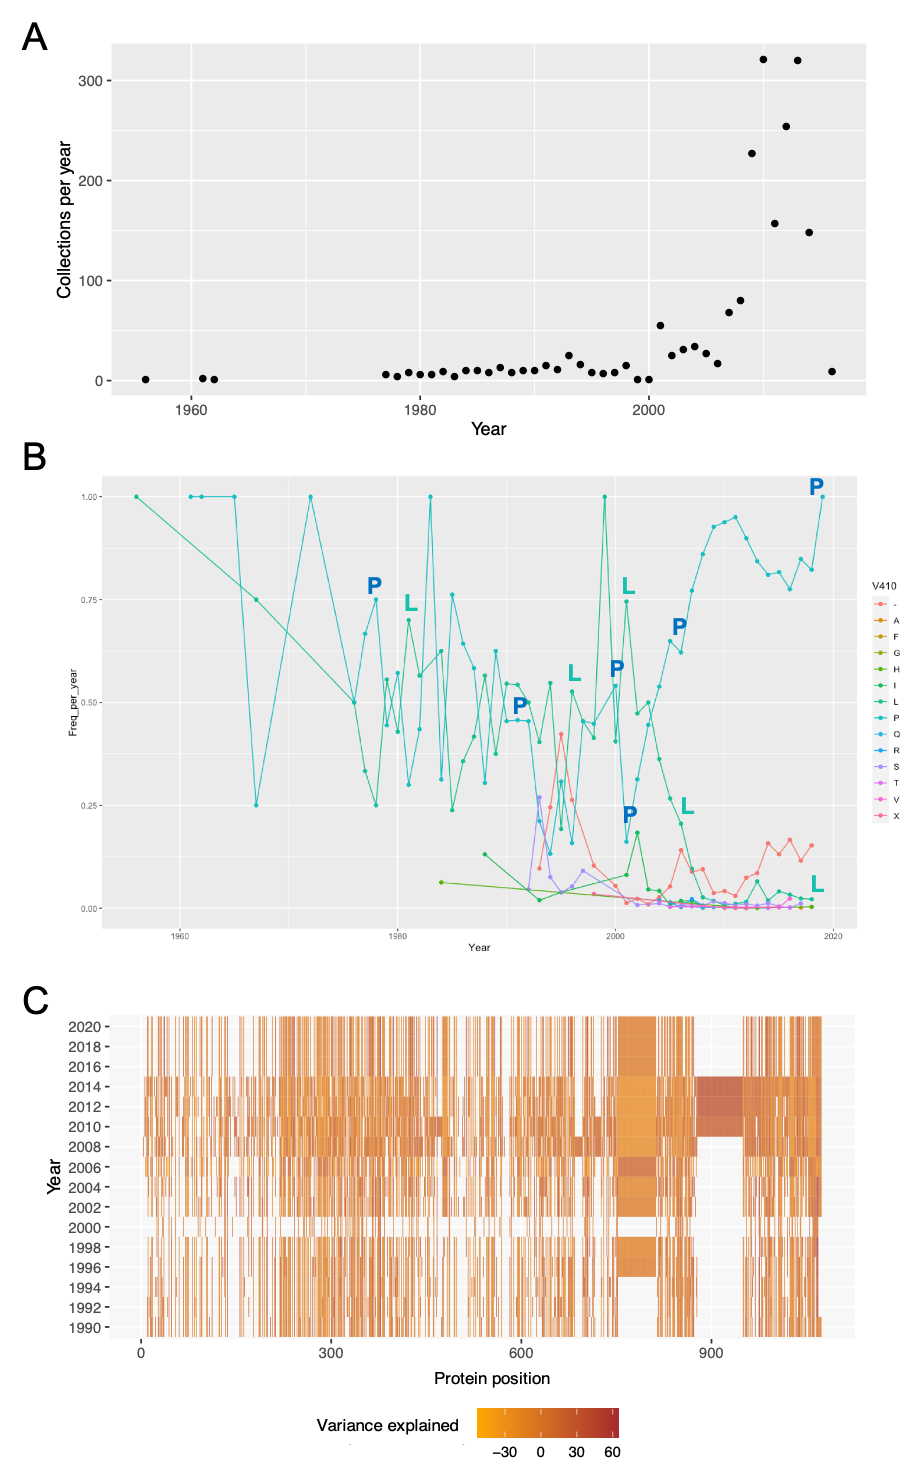
\includegraphics[scale=0.6]{S2}
	\caption{\textbf{Supplemental: Publicly available RSV sequence data for $>30$ years}. (A) Global sample collection per year. (B) Variant associated with prolonged infection tracked in public data. (C) \% variance explained per year for all G protein amino acid variants from 1990-2022} 
	\label{fig:S2} \end{center}
\end{figure}


\end{document}

